\documentclass[11pt,twoside]{scrartcl}
\usepackage{mdas}
% \usepackage[sexy, fancy, hints]{evan}
\begin{document}
\title{How to Use Tikz}
% If you contribute to the handout, put your name in comment here

\author{manojdas1@gmail.com}
\org{Manoj Latex Notes}
\date{\today}

\maketitle

\begin{abstract}
    Usage examples for Tikz. 
\end{abstract}

\section{Examples}

\subsection{Bipartite Graph}
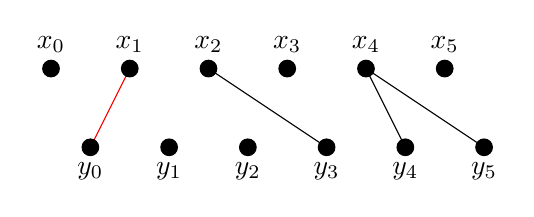
\begin{tikzpicture}
    \draw[red] (.5,0) -- (1,1);
    \draw (2,1) -- (3.5,0);
    \draw (4,1) -- (4.5,0);
    \draw (4,1) -- (5.5,0);
    \foreach \x in {0,...,5}
    {
        % \draw (\x,0) circle (3pt);

        \filldraw (\x, 1) circle (3pt);
        \path node at (\x, 1.3) {$x_{\x}$};
        \filldraw (\x + 0.5, 0) circle (3pt);
        \path node at (\x + 0.5, -.3) {$y_{\x}$};
    }
\end{tikzpicture}

\subsection{Markov Chain}
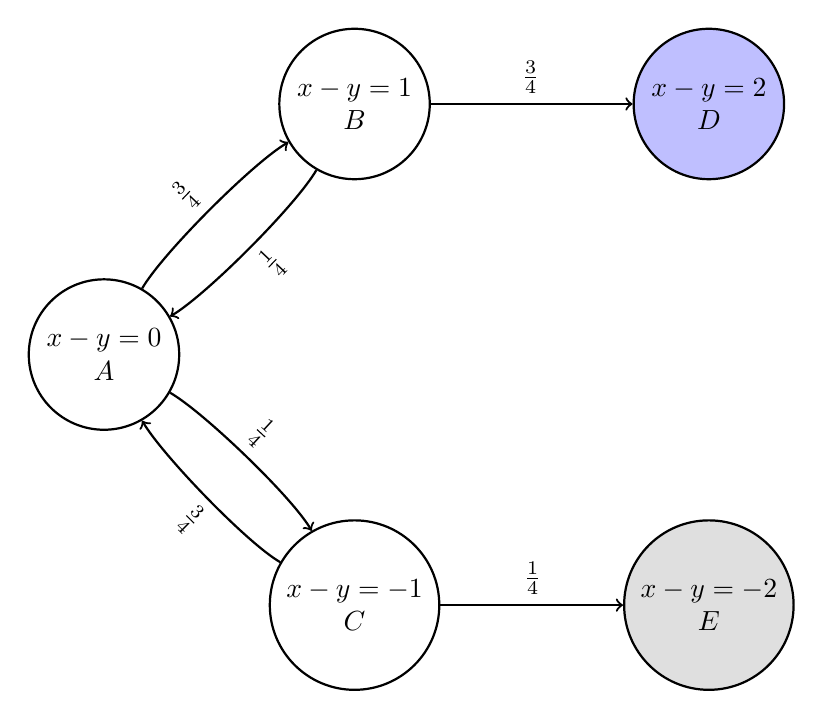
\begin{tikzpicture}[node distance={45mm}, thick, main/.style = {draw, circle}] 
    \node[main, align=center] (1) {$x-y=0$\\$A$}; 
    \node[main, align=center] (2) [above right of=1] {$x-y=1$\\$B$}; 
    \node[main, align=center] (3) [below right of=1] {$x-y=-1$\\$C$}; 
    \node[main, align=center] (4) [right of=2, fill=blue!25] {$x-y=2$\\$D$}; 
    \node[main, align=center] (5) [right of=3, fill=gray!25] {$x-y=-2$\\$E$}; 
    \draw[->] (1) to [out=60, in=210, looseness=.5] node[midway, above right, sloped, pos=0.4] {$\frac{3}{4}$}(2); 
    \draw[->] (2) to [out=240, in=30, looseness=.5] node[midway, below left, sloped, pos=0.4] {$\frac{1}{4}$}(1); 
    \draw[->] (1) to [out=-30, in=120, looseness=.5] node[midway, above right, sloped, pos=0.4] {$\frac{1}{4}$}(3); 
    \draw[->] (3) to [out=150, in=-60, looseness=.5] node[midway, below left, sloped, pos=0.4] {$\frac{3}{4}$}(1); 

    \draw[->] (2) to node[midway, above right, sloped, pos=0.4] {$\frac{3}{4}$}(4); 
    % \draw[->] (4) to [out=195, in=-15, looseness=.5] node[midway, above right, sloped, pos=0.6] {+2}(2); 

    \draw[->] (3) to  node[midway, above right, sloped, pos=0.4] {$\frac{1}{4}$}(5); 
    % \draw[->] (5) to [out=195, in=-15, looseness=.5] node[midway, above right, sloped, pos=0.6] {+2}(3); 
    % \draw[->] (6) -- node[midway, above right, sloped, pos=1] {+1} (4); 
\end{tikzpicture} 

\end{document}